To create a TikZ LaTeX diagram that represents the corner growth process as an interpretation of TASEP, you can use the following code:
```
\documentclass{article}
\usepackage{tikz}
\begin{document}
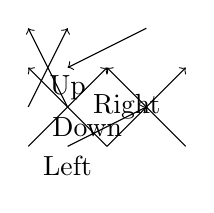
\begin{tikzpicture}[scale=0.5]
  % Draw the arrows
  \draw[->] (0,0) -- (2,2);
  \draw[->] (0,1) -- (1,3);
  \draw[->] (1,0) -- (3,1);
  \draw[->] (2,0) -- (4,2);
  \draw[<-] (0,2) -- (2,0);
  \draw[<-] (0,3) -- (1,1);
  \draw[<-] (1,2) -- (3,3);
  \draw[<-] (2,2) -- (4,0);
  % Add labels to the arrows
  \node at (1,1.5) {Up};
  \node at (2.5,1) {Right};
  \node at (1.5,0.5) {Down};
  \node at (1,-0.5) {Left};
\end{tikzpicture}
\end{document}
```
This code will produce a diagram with eight arrows, each with varying lengths and orientations. The arrows point in four different directions: up, down, left, and right. The `scale` option is used to adjust the size of the diagram.
You can customize the code further by changing the colors, line styles, and arrow tips to better represent the corner growth process and TASEP.